\chapter{Simulations of Magnetic ripple}
\label{chap:RippleMagnetic}

Developments performed in the scope of this thesis can be useful for applications other than electromagnetic effects on plasmas. In transport mode with large perpendicular diffusion coefficients, a regime where drifts and turbulent scales are not solved, modulations of the magnetic field can have an external source. Because of the toroidal locality of toroidal field coils, the equilibrium magnetic field itself is not axisymmetric, a phenomenon usually referred to as "magnetic ripple". This chapter describes how the implementation of fluctuating magnetic fields in the framework of flutter can be used to simulate perturbations of the equilibrium magnetic field.

\section{Motivation for simulating magnetic ripple}\label{sec:ripple_intro}

Power exhaust is a major concern in magnetic fusion research. Accurately predicting the heat load on the divertor plates is essential for the design and operation of current and future tokamaks. Estimates for the International Thermonuclear Experimental Reactor (ITER), the most powerful device currently under construction, indicate maximum local heat loads close to material limits\cite{gunn2017surface}.For this reason it is important to study transport of heat and particle fluxes in present experiments, coupling the experimental analysis with a modelling effort  with dedicated numerical tools. \newline

Experiments conducted on the tungsten environment steady-state tokamak (WEST) at CEA in Cadarache, France\cite{bucalossi2022}, have demonstrated that the heat deposition on the divertor targets is not uniform in the toroidal direction. A "snake skin" pattern (see Figure \ref{fig:IR_WEST}), with alternating local maxima, appears on the inner and outer divertor targets. Reconstructions from infrared camera images exhibit a considerable difference between peaks and lows along a target line. These variations correlate with the disposition of the toroidal magnetic field coils, which locally modify the field lines and amplitude. This effect is known as magnetic ripple\cite{tani1981effect}, and it is particularly pronounced on WEST, where the 18 coils cause strong variations in the amplitude of the magnetic field $\textbf{B}$. For example, fast ions trapped in the toroidal magnetic field ripple have been found to be responsible for significant power losses\cite{moiraf2023optimization}. Moreover, it is important to determine the impact of this toroidal modulation on impurity transport, in particular on tungstene contamination of the core\cite{diGenova2021modelling}. \newline

SOLEDGE3X is a powerful fluid code for scrape-off-layer (SOL) and edge plasma analysis. The simulation domain extends from the far core across the separatrix up to the first wall in complex geometries. Its full model is capable of simulating resistive drift-wave turbulence\cite{bufferand2017} with advanced fluid closures\cite{bufferand2022implementation} and interactions with recycling neutrals\cite{quadri2024}. A "transport" mode, where cross-field transport is approximated with effective diffusion coefficients, allows simulations to run until convergence on large machines like ITER\cite{rivals2022soledge3x} or JT-60SA\cite{deGianni2024}. Applications of this code include studies on impurity transport\cite{Ciraolo2021}, heat exhaust\cite{rivals2022impact}, and detachment regimes in the divertor\cite{yang2023control}. \newline


\begin{figure}[H]\centering
	\centering
	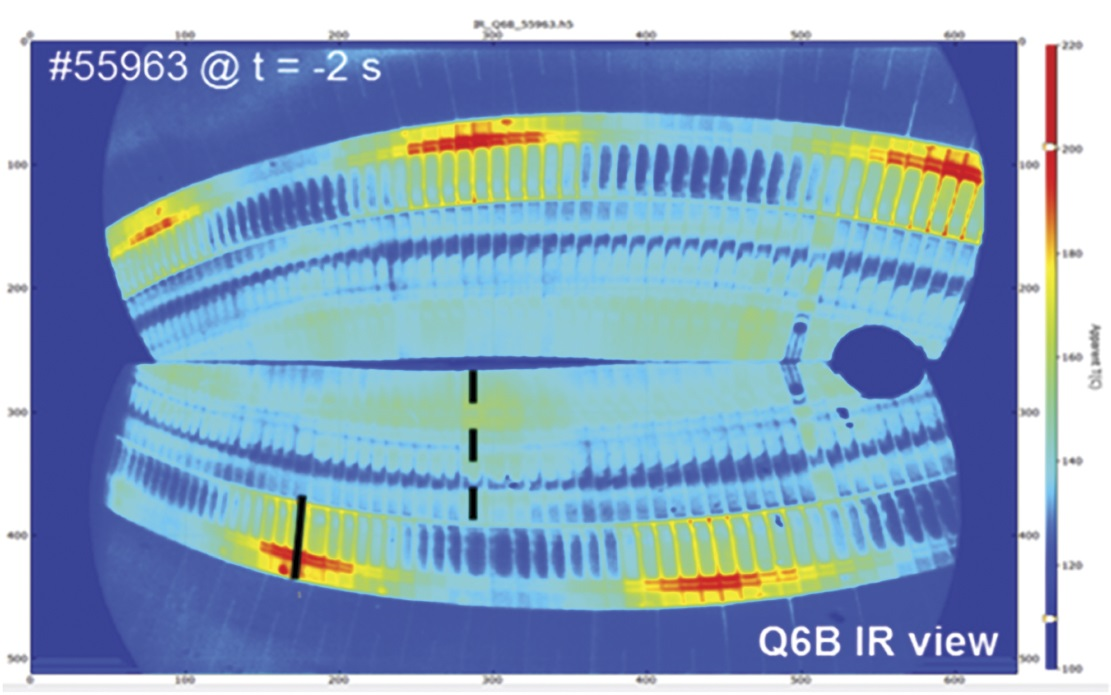
\includegraphics[width=0.48\textwidth]{schemes/IR_WEST_ripple.jpg}
	\caption{Infrared camera view of the divertor target, taken from \cite{bucalossi2022}. Red zones correspond to hot regions with high heat deposition. One can see the "snake skin" pattern, where the maximal intensity alternates between the inner and outer strike points.}
	\label{fig:IR_WEST}
\end{figure}

In its current form, SOLEDGE3X can address 2D and 3D axisymmetric configurations as well as 3D non axisymmetric wall geometries\cite{diGenova2023thesis}, but still requires a 3D axisymmetric magnetic field. Therefore, toroidal variations of the magnetic field due to ripple could not be taken into account. Moreover, matching simulation results to experimental data is made difficult by the toroidal locality of Langmuir probes and their consequent susceptibility to ripple effects. Recent developments in the turbulence model have introduced electromagnetic effects\cite{dull2024introducing}, where magnetic field lines are perturbed by fluctuations of the magnetic vector potential. In this paper, we demonstrate that the new implementations can be used not only for plasma-induced perturbations but also for external perturbations of the axisymmetric magnetic field. This paves the way for ripple simulations in SOLEDGE3X and will be applied to a WEST scenario in this paper. 

\section{Generation of a non-axisymmetric magnetic configuration}
\label{sec:rippleCalculation}

The SOLEDGE3X framework is capable of addressing magnetic configurations with singularities at one or more X-points. Constructed by a combination of a toroidal field, $\textbf{B}_t$, and a poloidal field, $\textbf{B}_{pol}$, the expression for the magnetic field is:

\begin{equation}
	\textbf{B}_{axi} = \textbf{B}_t + \textbf{B}_{pol} = F\grad{\varphi} + \grad{\Psi}\cross\grad{\varphi} \label{eq:axiSymBfield}
\end{equation}

where $\varphi$ represents the toroidal angle. The toroidal field $\textbf{B}_t$ is derived from a toroidal flux $F$ and $\textbf{B}_{pol}$ from a poloidal flux function $\Psi$. For high numerical accuracy, the meshing in SOLEGE3X is aligned to magnetic flux surfaces, treating singularities with a multi-domain decomposition shown in Figure \ref{fig:WESTmesh} \newline 

\begin{figure}[H]\centering
	\centering
	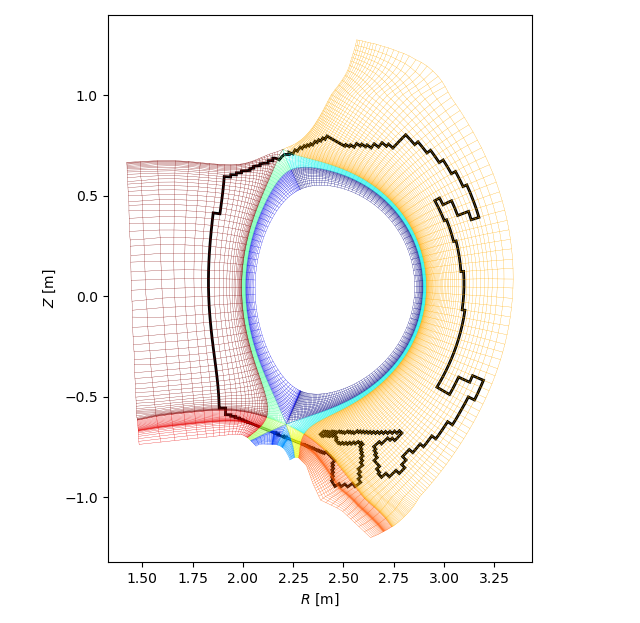
\includegraphics[width=0.48\textwidth]{schemes/WESTmesh.png}
	\caption{Exemplary SOLEDGE3X mesh for a WEST single-null geometry }
	\label{fig:WESTmesh}
\end{figure}

On top of this axisymmetric basis, we calculate the ripple perturbation of the magnetic field induced by the toroidal distribution of the toroidal field coils. For that, we simplify each coil to a single, circular wire. We first discretize each of the $N_{c}$ coils into $N_{seg}$ segments. For every cell in the SOLEDGE3X grid, we then calculate the magnetic field associated with the coils using the Biot-Savart law:

\begin{equation}
	\textbf{B}_{ripple} = \frac{\mu_0}{4\pi}I_c\sum_{i=1}^{N_{c}}\sum_{j=1}^{N_{seg}}\frac{\textbf{d}_{i,j}\cross\left(\textbf{s}_{i,j+1} - \textbf{s}_{i,j}\right)}{\norm{\textbf{d}_{i,j}}^3}
\end{equation}

where the coil current $I_c$ corresponds to the nominal coil current times the number of wire turns in a coil, $\textbf{s}_{i,j}$ represents the start and end locations of each coil segment, and $\textbf{d}_{i,j}$ is the vector from each mesh point to the segment center. To avoid accounting for the axisymmetric component of the magnetic field twice, we define the perturbation field as the toroidal fluctuations of the ripple field:


\begin{equation}
	\textbf{B}_{pert} = \textbf{B}_{ripple} - \left<\textbf{B}_{ripple}\right>_\varphi
\end{equation}


Together with the axisymmetric part from Equation \ref{eq
}, the equilibrium magnetic field as applied to the simulation is given by:

\begin{equation}
	\textbf{B} = \textbf{B}_{axi} + \textbf{B}_{pert}
\end{equation}

\begin{figure}[H]
	\centering
	\begin{subfigure}[t]{0.3\textwidth}
		\centering
		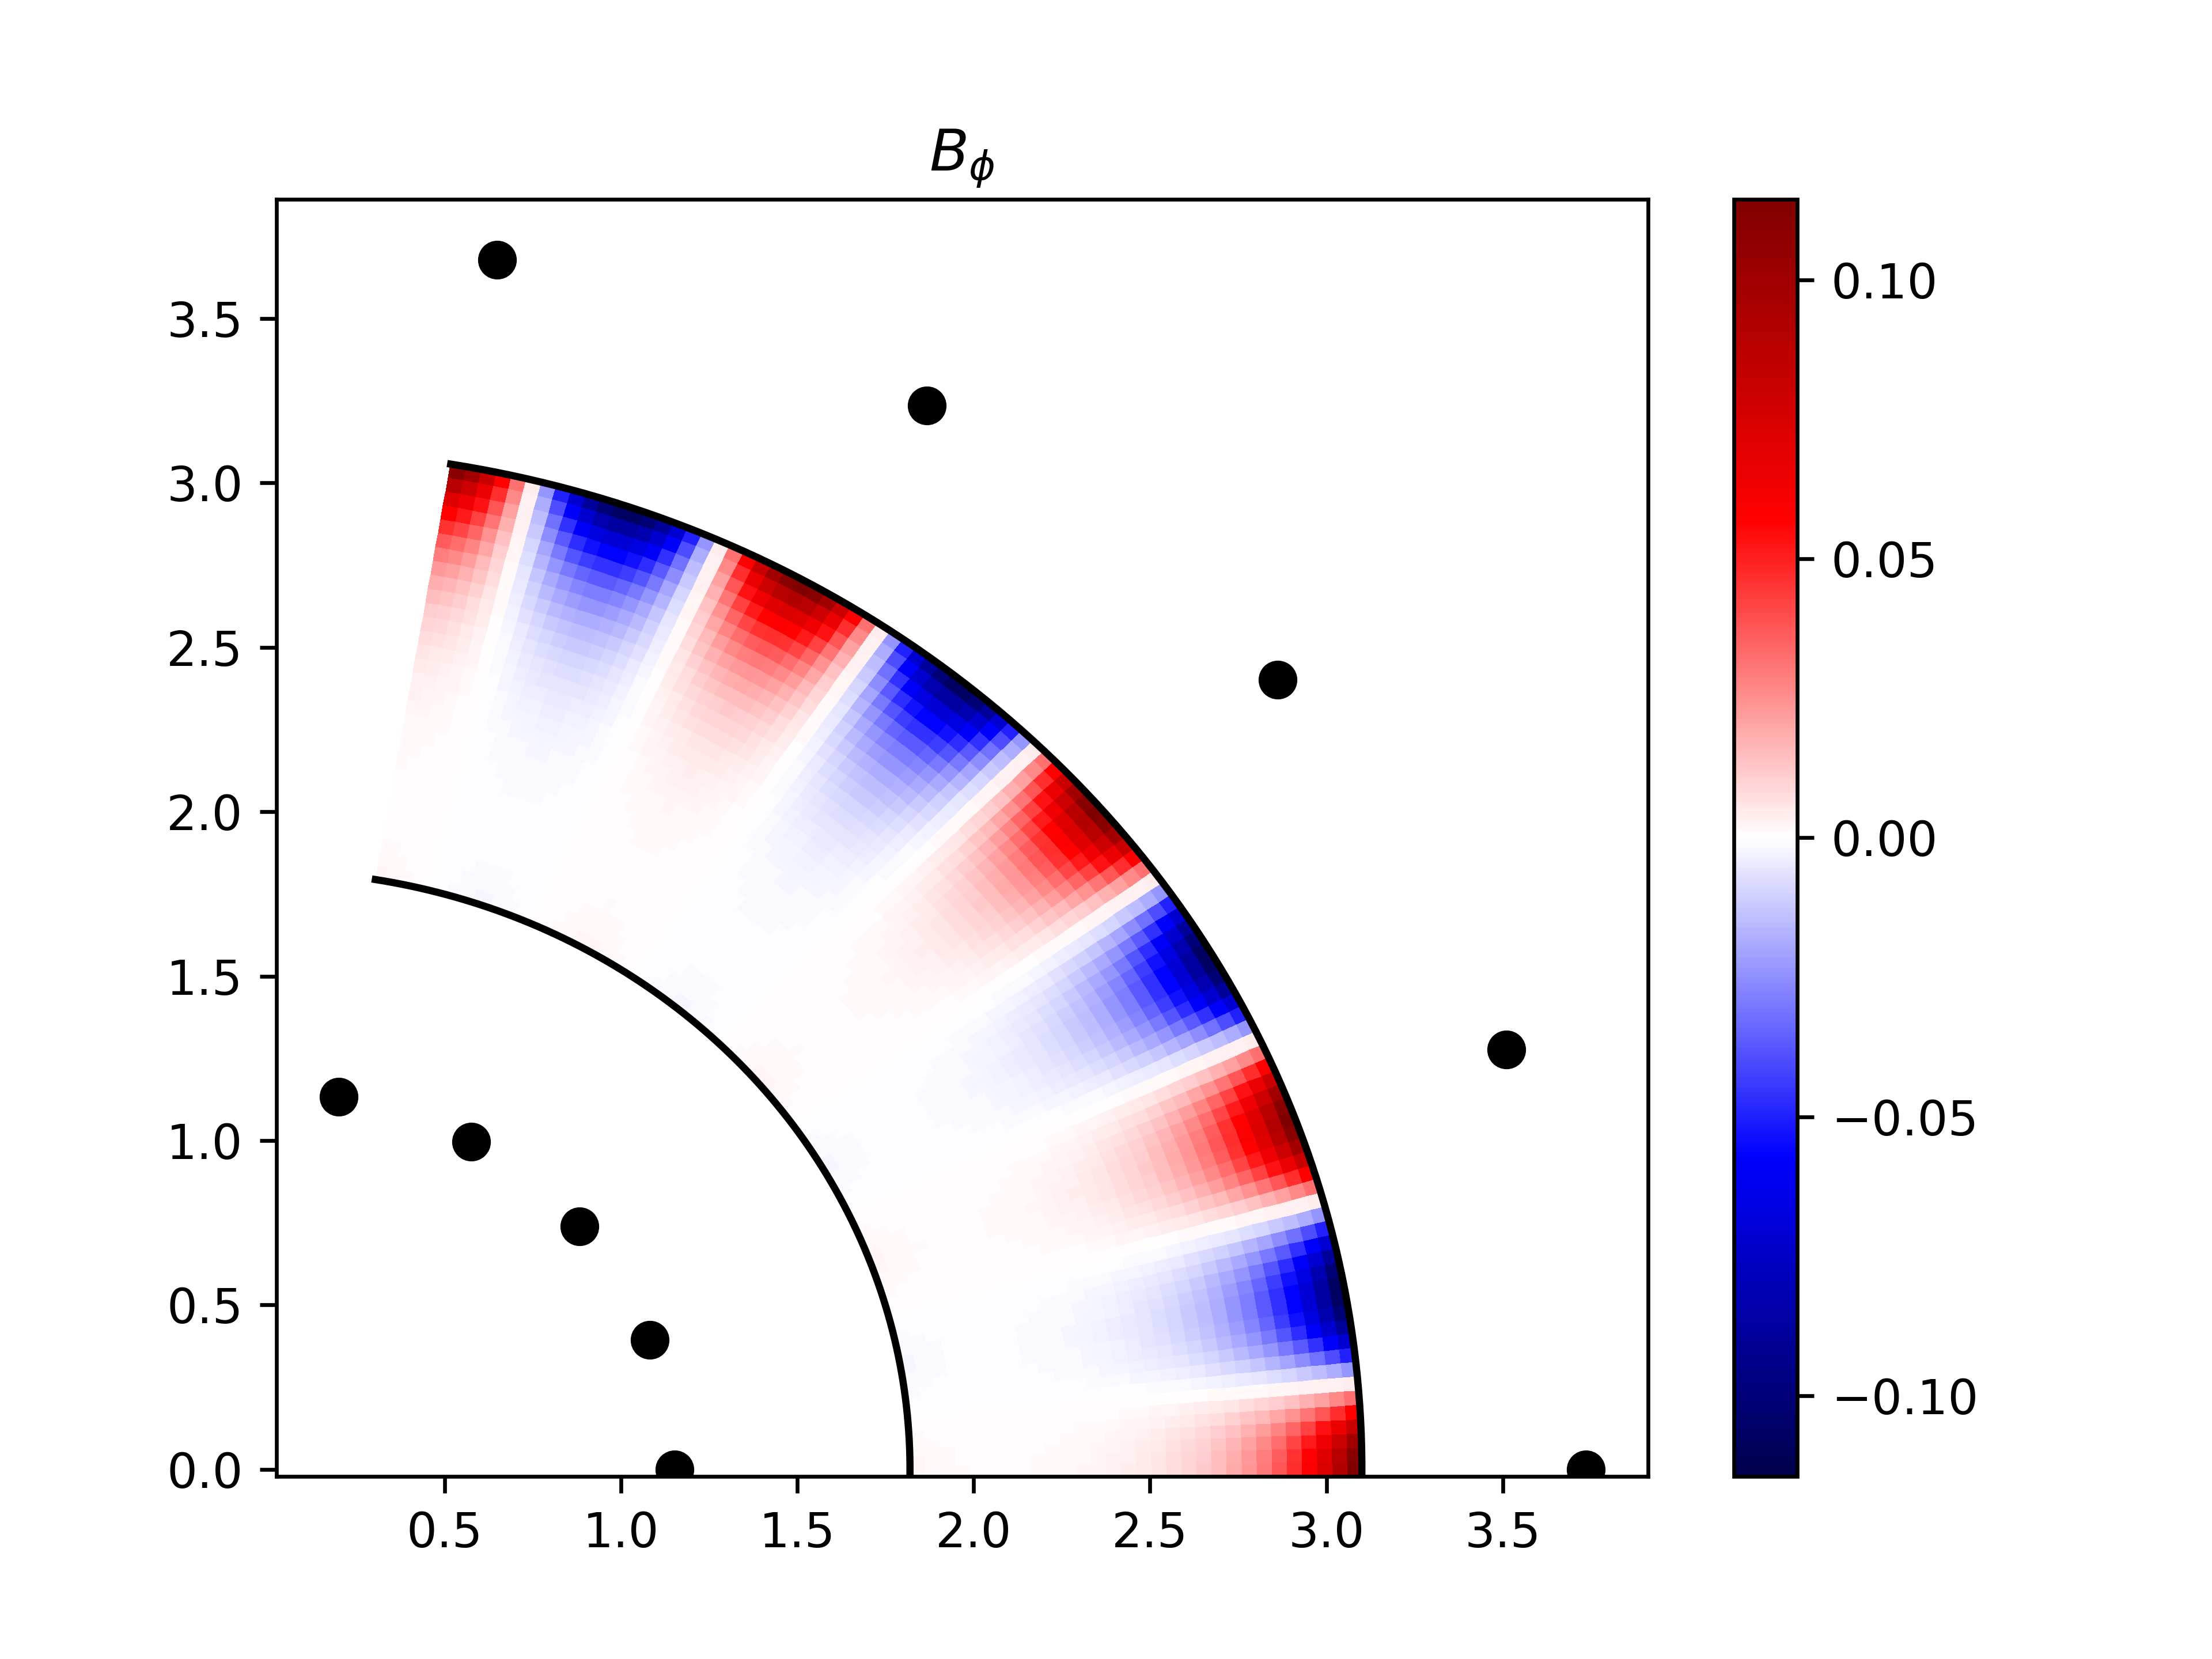
\includegraphics[width=1\textwidth]{schemes/rippleBphi.png}
		\subcaption{toroidal component $B_{pert}^\varphi$ }
		\label{fig:Bpert_phi}
	\end{subfigure}
	\begin{subfigure}[t]{0.3\textwidth}
		\centering
		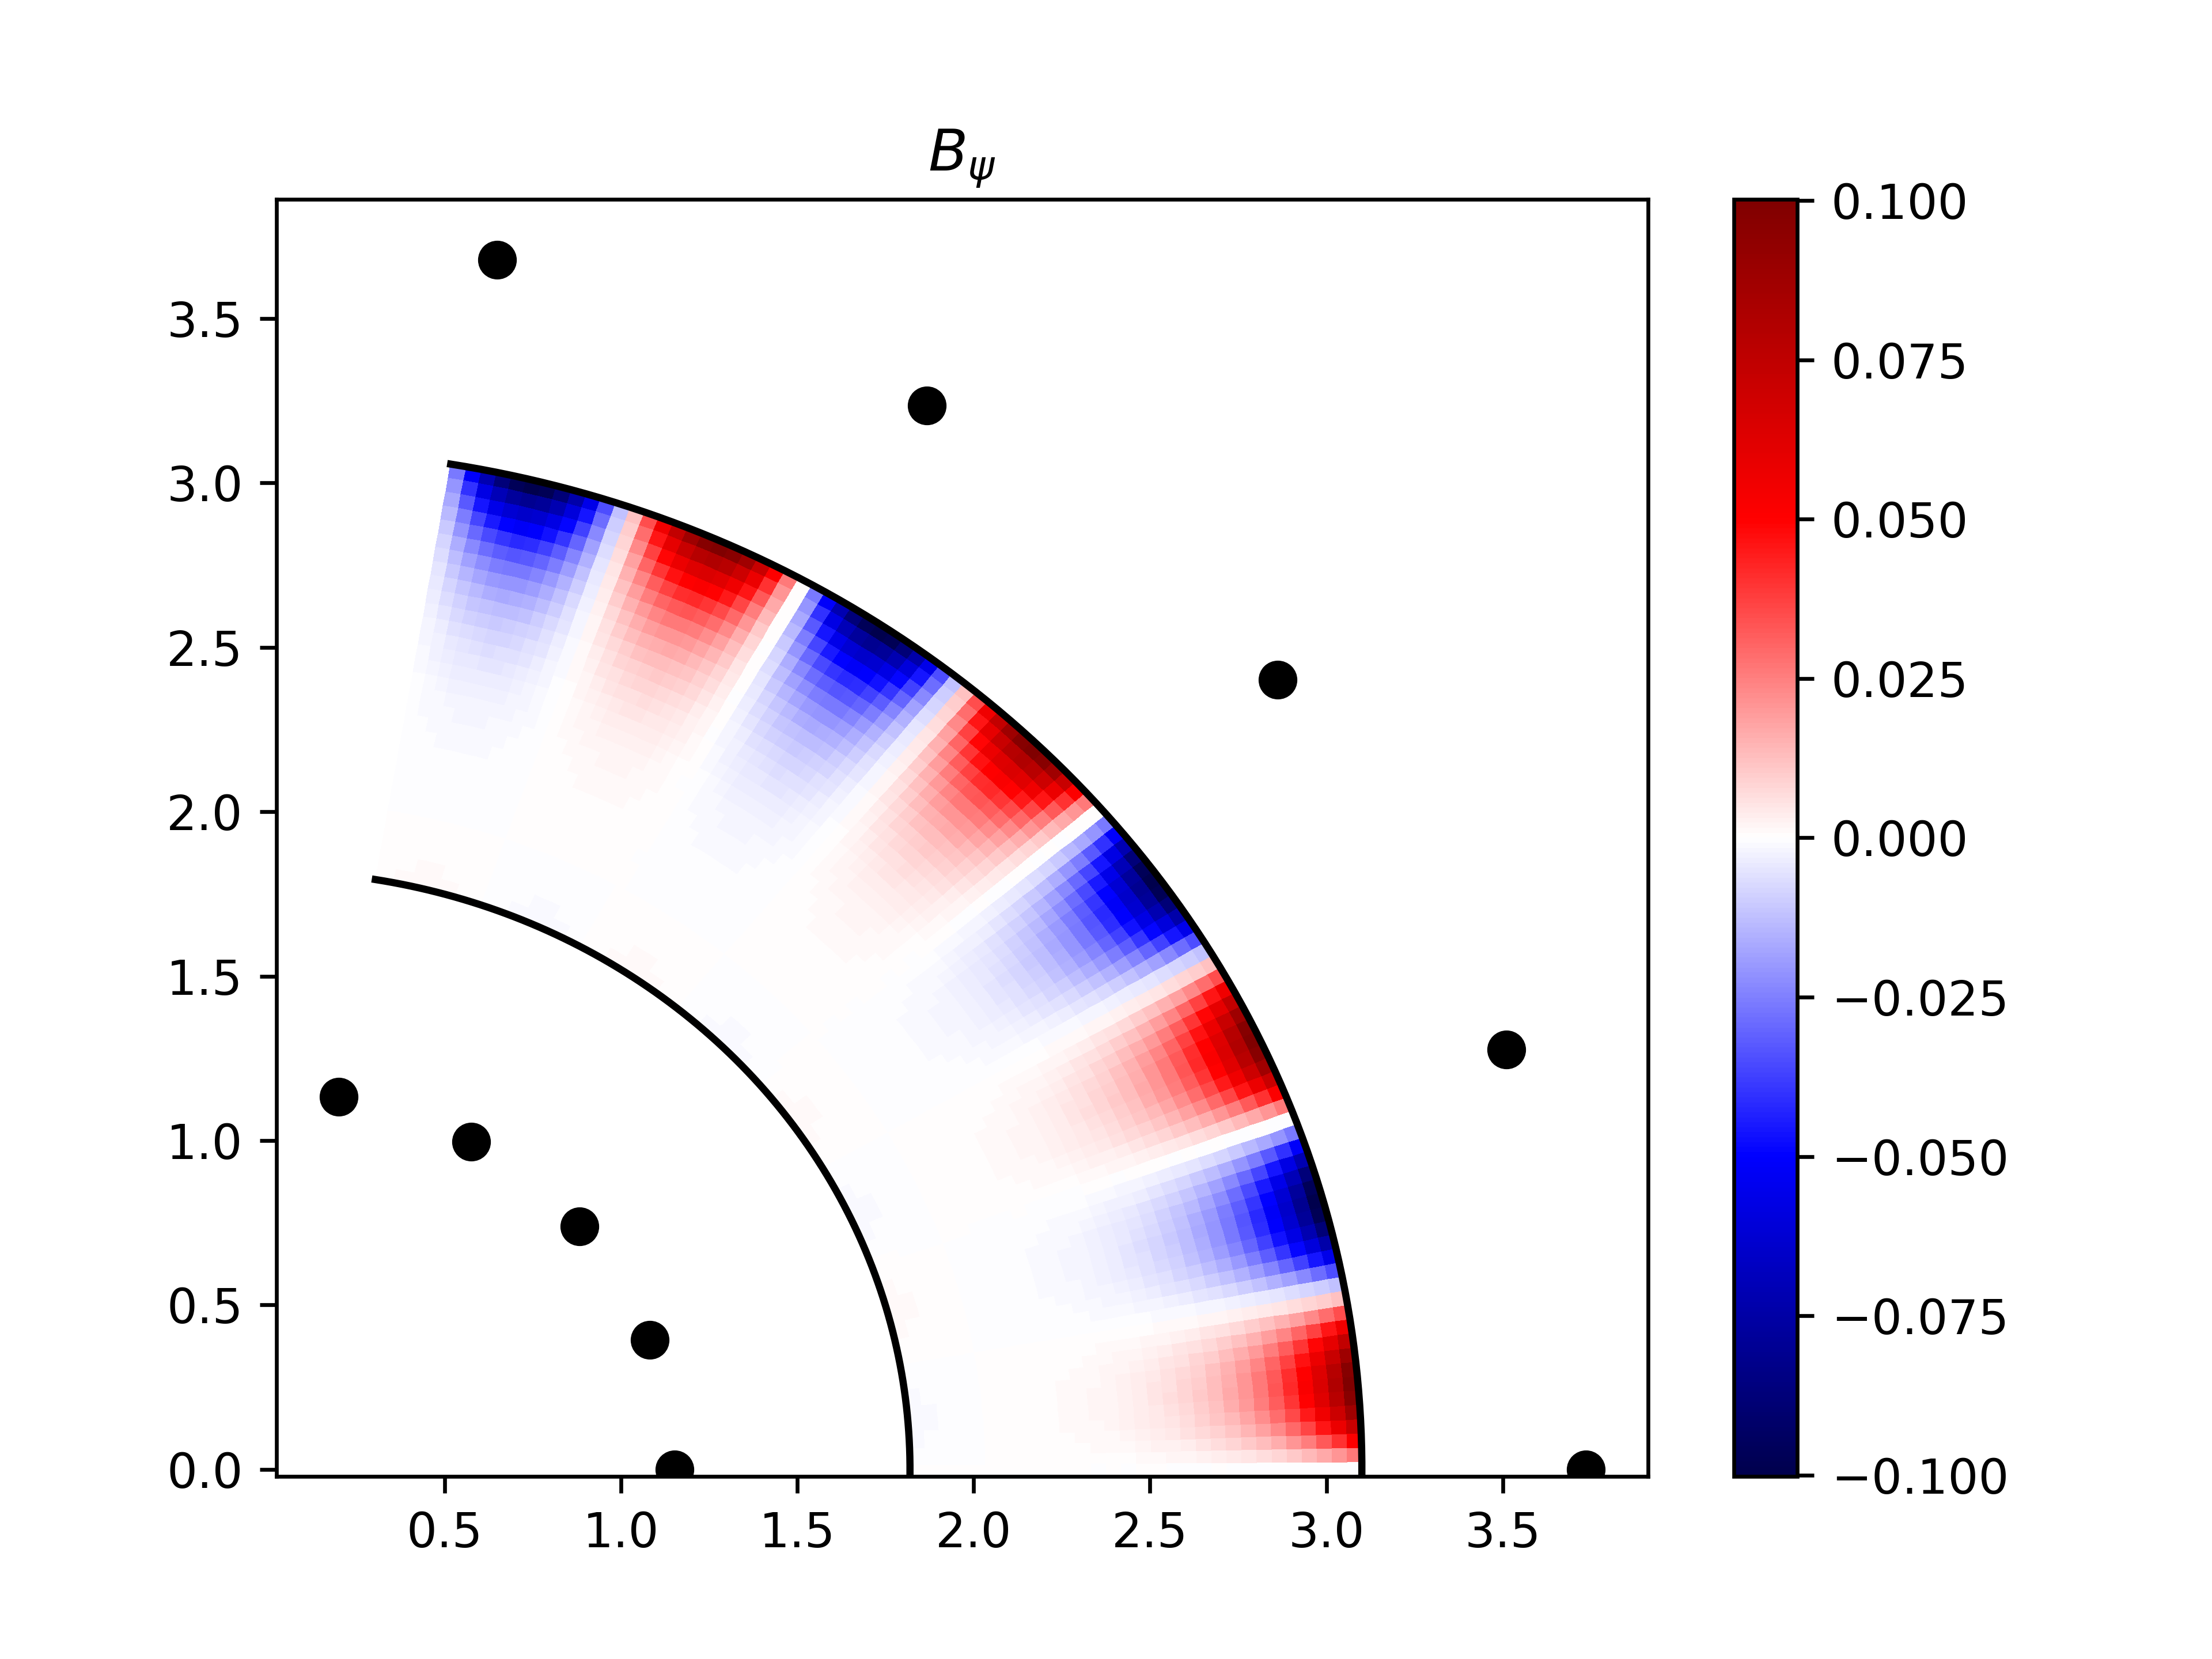
\includegraphics[width=1\textwidth]{schemes/rippleBpsi.png}
		\subcaption{radial component $B_{pert}^\psi$ }		
		\label{fig:Bpert_psi}
	\end{subfigure}
	\begin{subfigure}[t]{0.3\textwidth}
		\centering
		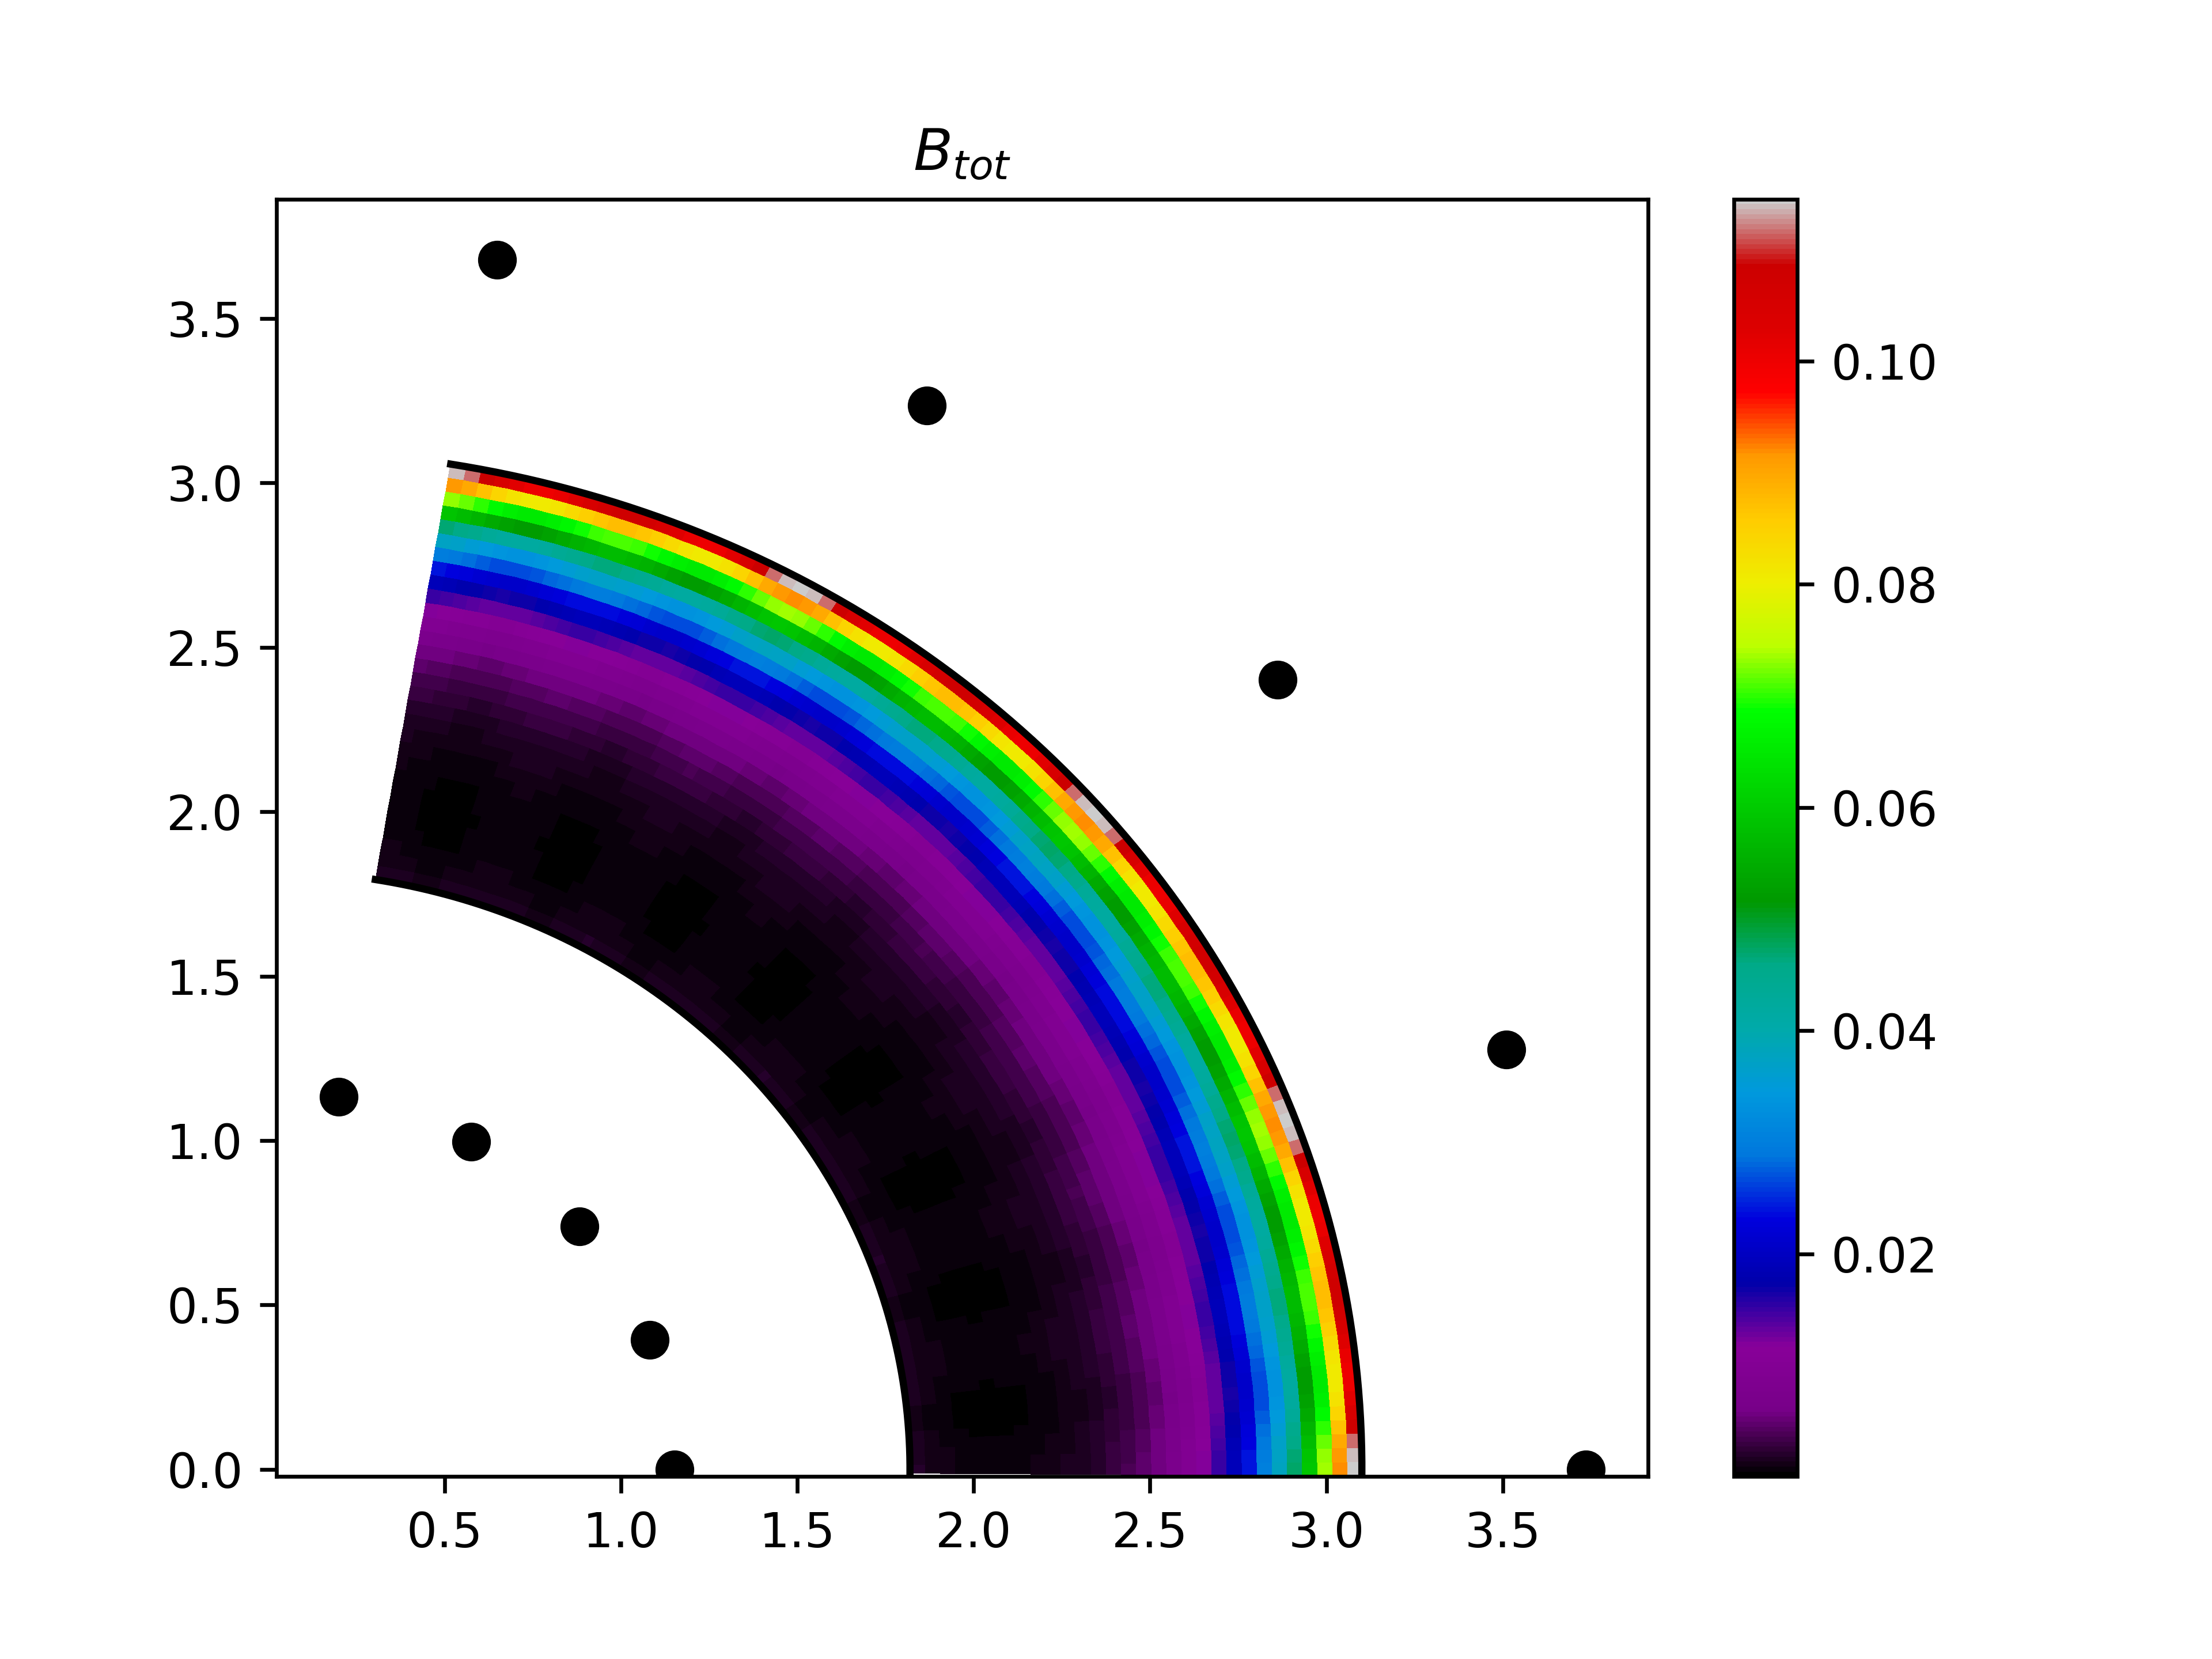
\includegraphics[width=1\textwidth]{schemes/rippleBtot.png}
		\subcaption{amplitude of the field $\norm{\textbf{B}_{pert}}$}
	\end{subfigure}
	\caption{Top views of the perturbated field $\textbf{B}_{pert}$ on the WEST tokamak at the mid plane. The black dots indicate the position of the toroidal field coils. The  amplitude of the perturbated field remains much smaller than the axisymmetric component, whose amplitude ranges around 1T.}
	\label{fig:Bpert_fields}
\end{figure}

This strategy is now applied to compute the magnetic field ripple for the WEST tokamak, with the coil parameters described in Table \ref{tab:coilParameters}. The ripple has a twofold impact on the magnetic equilibrium. A toroidal perturbation field, as shown in Figure \ref{fig:Bpert_phi}, modifies $\textbf{B}_t$ with local maxima located at the coils' positions and minima midway between two coils. The perturbation vanishes at $\pi/2$ and $3\pi/2$ of a ripple period. Conversely, the radial perturbation in Figure \ref{fig:Bpert_psi} vanishes at the coils and midway, and modifies the poloidal field $\textbf{B}_{pol}$.

\begin{table}[H]
	\centering
	\begin{tabular}{|c||c|c|}
		\hline
		Number of coils & $N_c$ & 18 \\
		\hline
		Major coil radius & $R_c$ & 2.443 m\\
		\hline
		Minor coil radius & $a_c$ & 1.292 m\\
		\hline
		Nominal coil current & $I_c$ & 1.2 kA \\
		\hline
		Number of wire turns & $N_{turns}$ & 2028 \\
		\hline        
	\end{tabular}
	\caption{Technical parameters of the toroidal field coils used to generate the ripple field for the WEST tokamak}
	\label{tab:coilParameters}
\end{table}

Even if the amplitude of the ripple field is small compared to the axisymmetric one, it strongly impacts the poloidal field $\textbf{B}_{pol}$ from one poloidal plane to another. As $\textbf{B}_{pol}$ approaches zero at X-points, the radial perturbation $\textbf{B}_{pert}^{\psi}$ induced by the coils dominates over the axisymmetric component. In Figure \ref{fig:ripple_Xpoint}, we observe that the X-point based on $B_{pol}$ shifts by about 4.1 cm towards the high-field side at the maximal radial perturbation and by 2.7 cm inwards at the minimum. \newline 


\begin{figure}[H]\centering
	\begin{subfigure}[t]{0.43\textwidth}
		\centering
		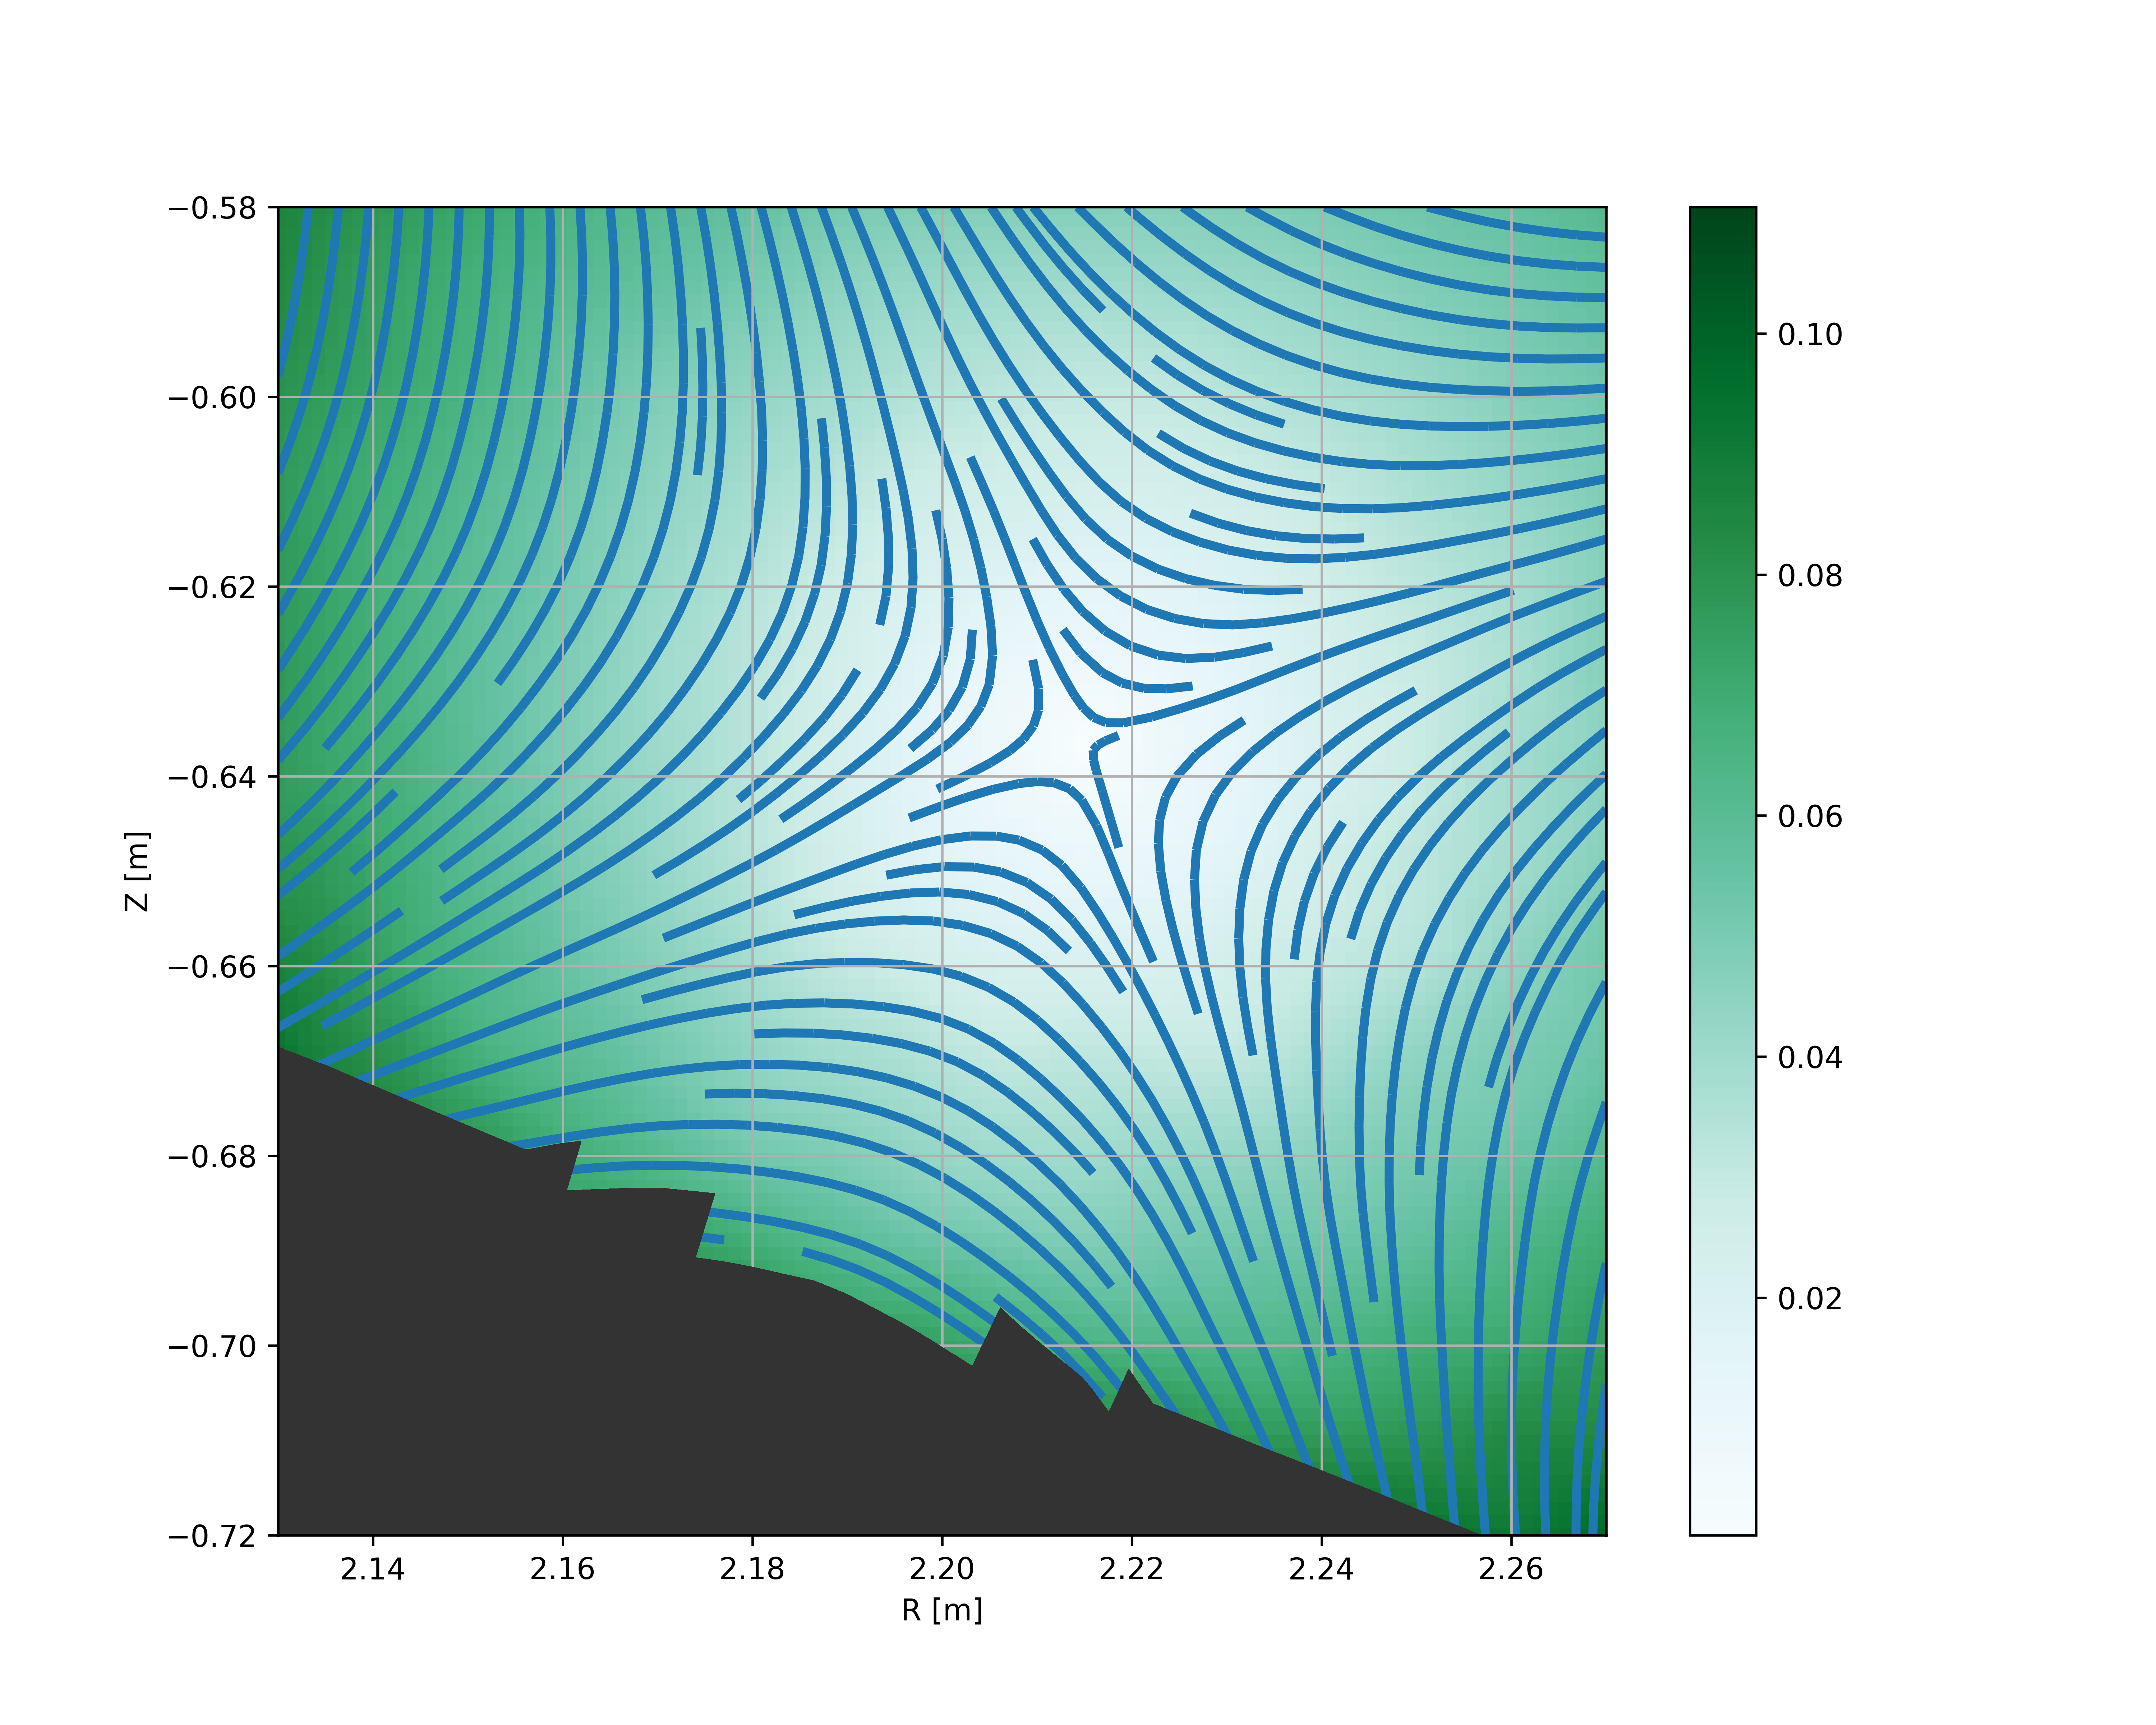
\includegraphics[width=1\textwidth]{schemes/rippleStreamlines_phi1.png}
		\subcaption{$0$}\label{fig:ripple_Xpoint_phi1}
	\end{subfigure}
	\begin{subfigure}[t]{0.43\textwidth}
		\centering
		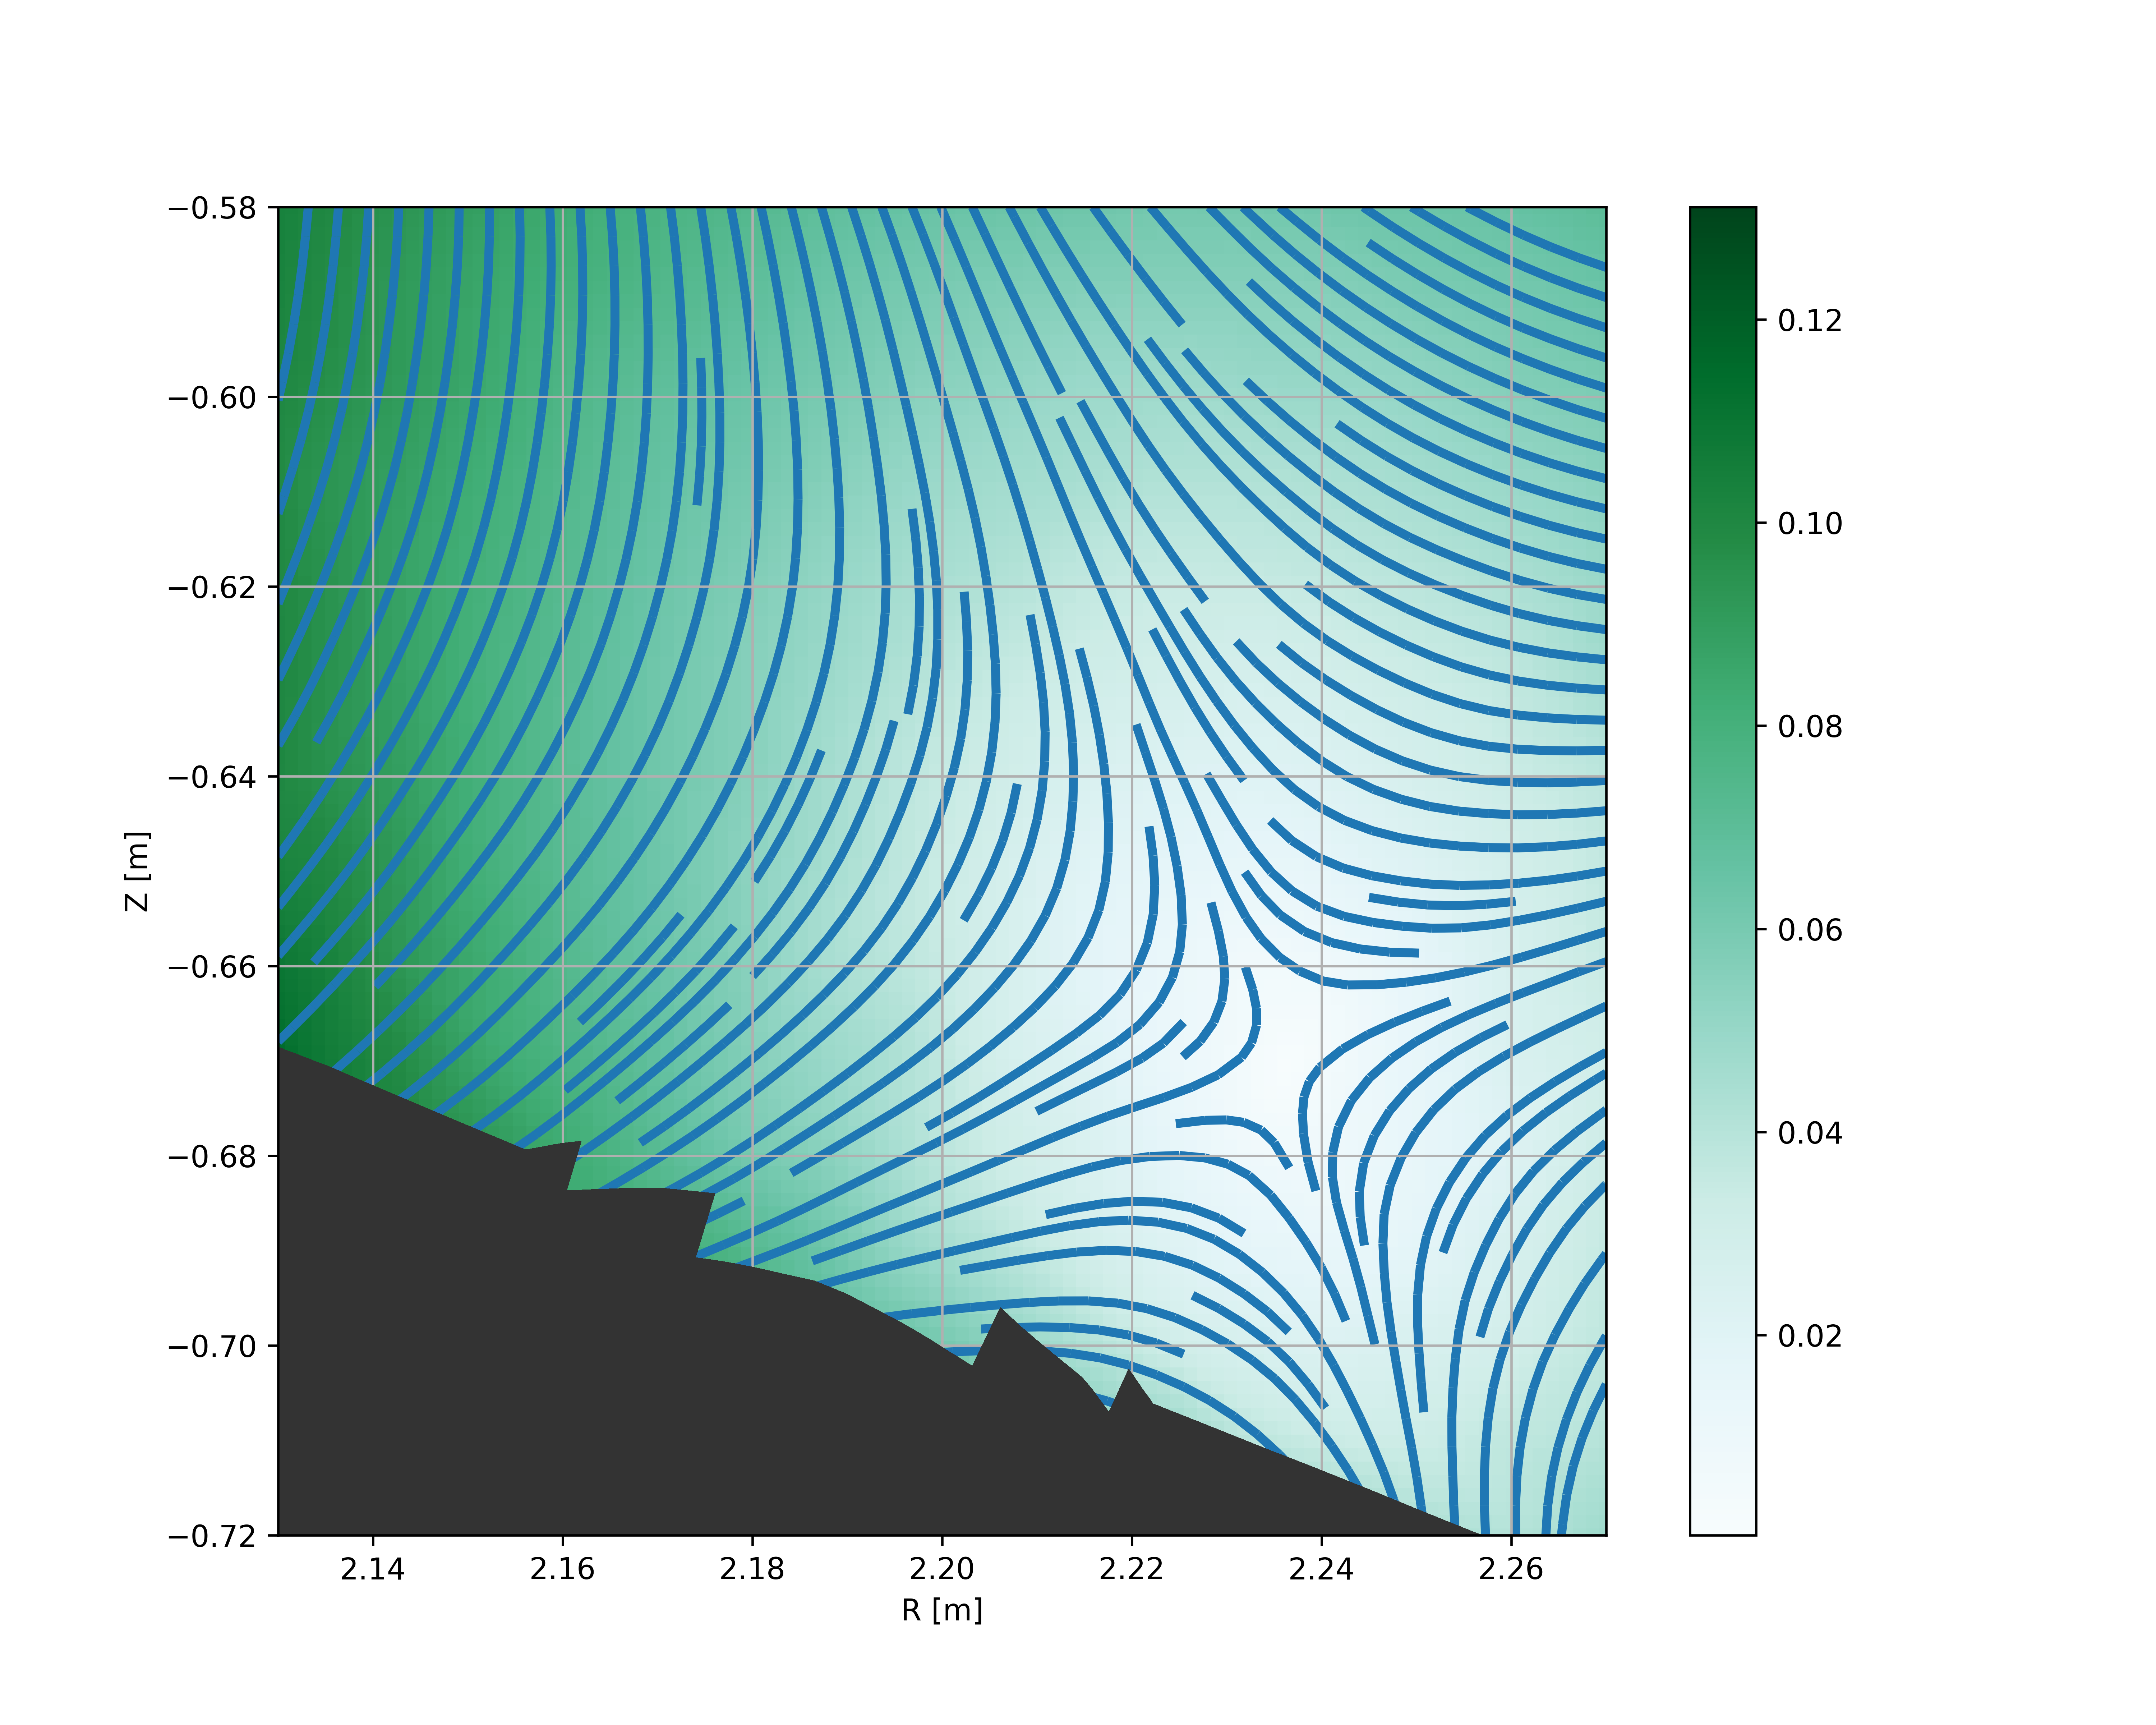
\includegraphics[width=1\textwidth]{schemes/rippleStreamlines_phi2.png}
		\subcaption{$1/4$}\label{fig:ripple_Xpoint_phi2}
	\end{subfigure}
	\begin{subfigure}[t]{0.43\textwidth}
		\centering
		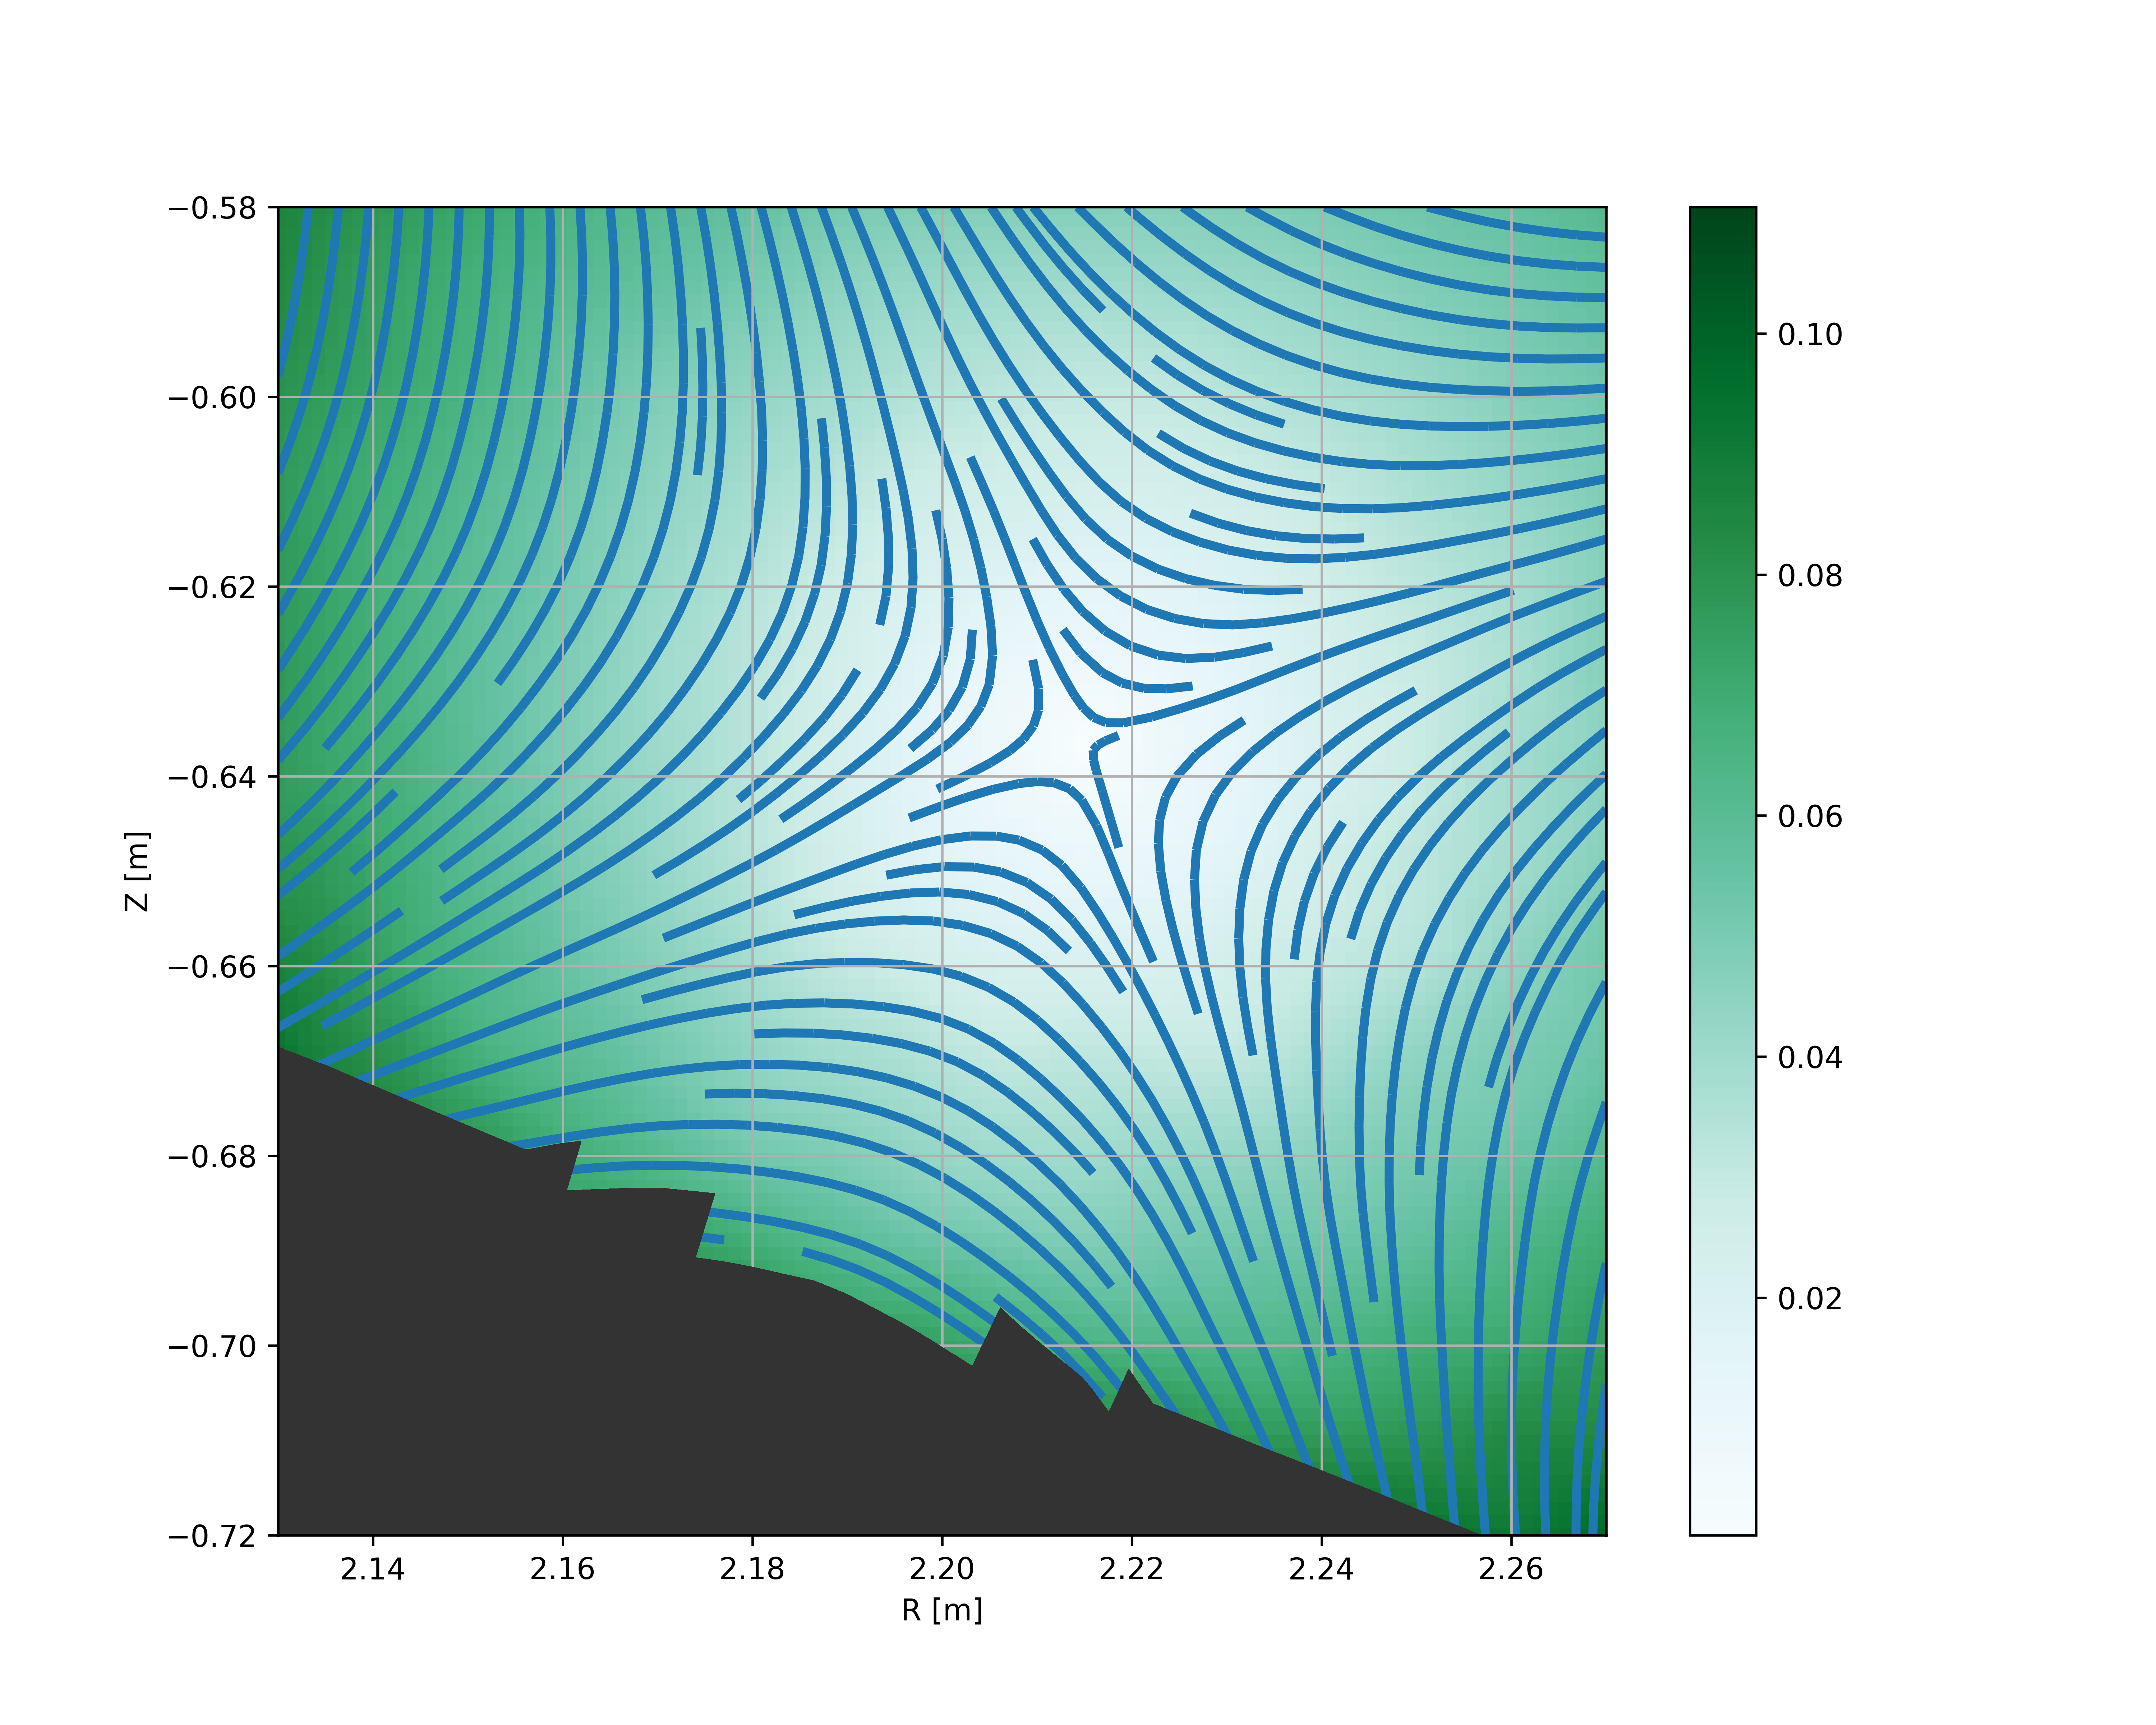
\includegraphics[width=1\textwidth]{schemes/rippleStreamlines_phi3.png}
		\subcaption{$1/2$}\label{fig:ripple_Xpoint_phi3}
	\end{subfigure}
	\begin{subfigure}[t]{0.43\textwidth}
		\centering
		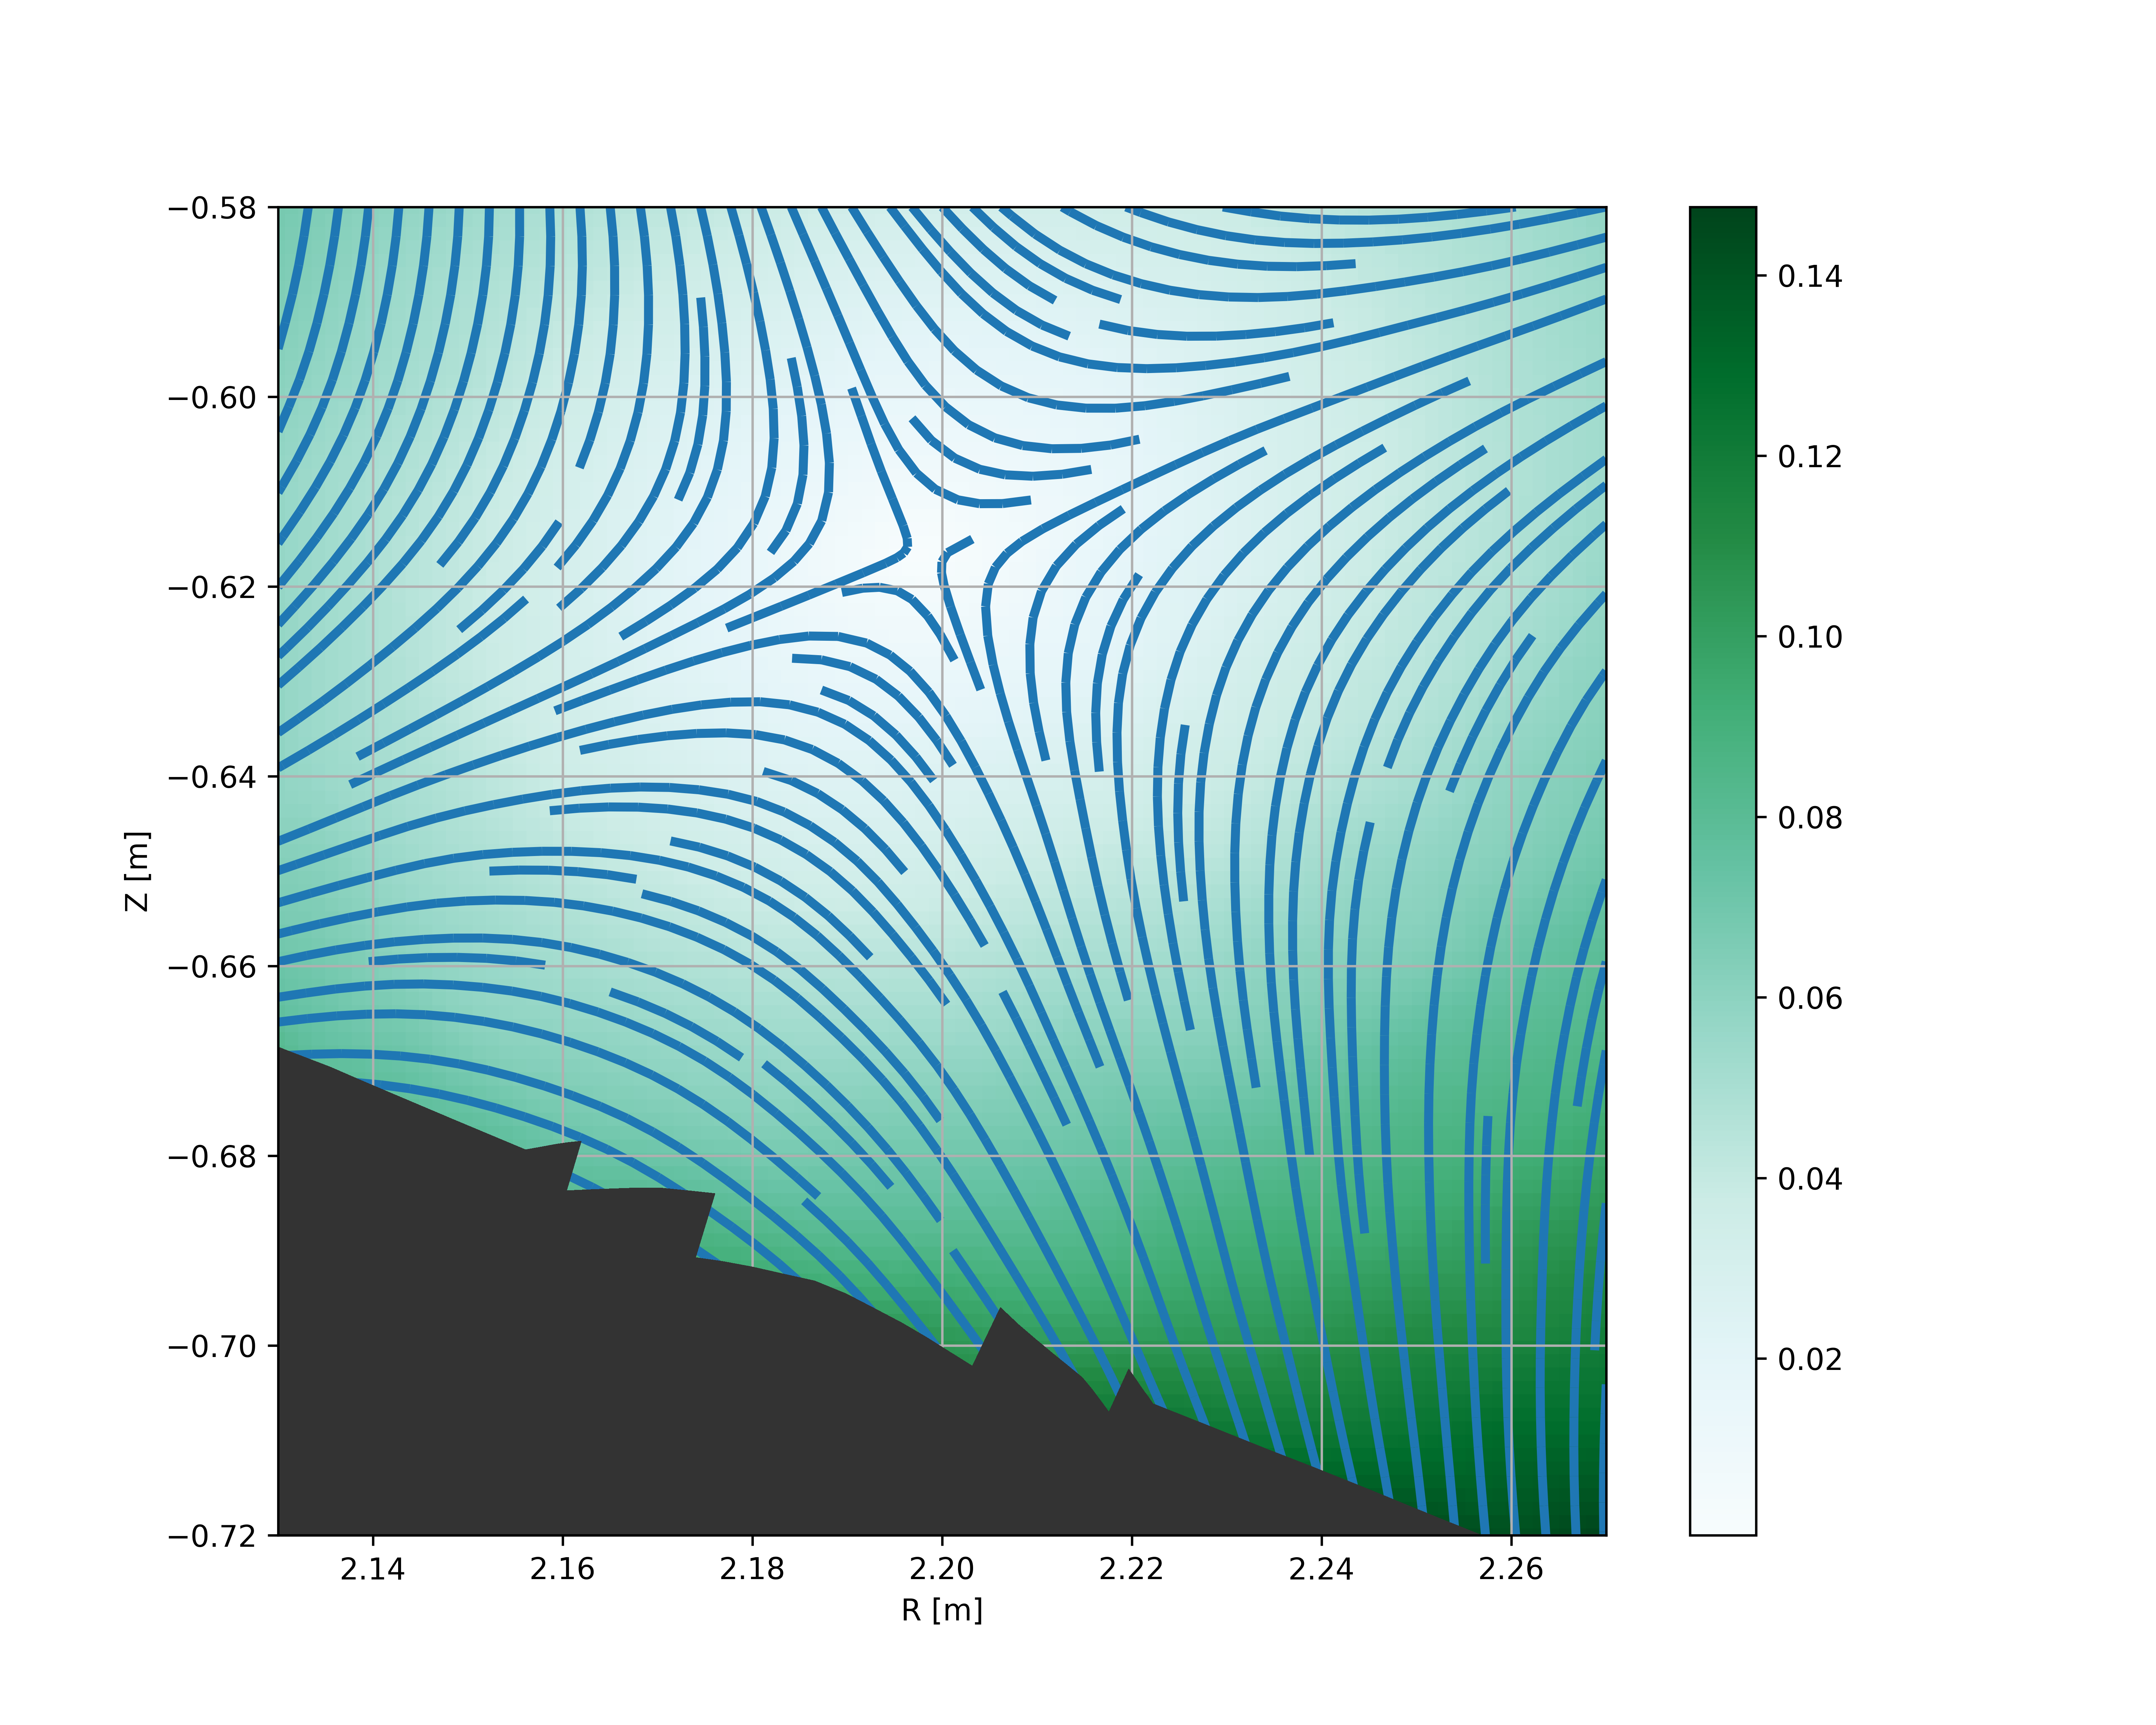
\includegraphics[width=1\textwidth]{schemes/rippleStreamlines_phi4.png}
		\subcaption{$3/4$}\label{fig:ripple_Xpoint_phi4}
	\end{subfigure}
	\caption{Map of the poloidal field $B_{pol}$ [T] at several poloidal planes within a ripple perdiod around the lower X-point and the divertor targets. Streamlines are supperposed to the fields to better visualize the position of the X-point and the separatrix at the divertor. The phase shifts $0$ and $1/2$ with respect to the coil positions are identical to the axisymmetric configuration as $B_{pert}^{\psi}$ vanishes while the planes at $1/4$ and $3/4$ correspond to the respective maximum and minimum of $B_{pert}^{\psi}$}
	\label{fig:ripple_Xpoint}
\end{figure}

However, this does not mean that the last closed flux surface (LCFS) experiences such a strong modulation. Indeed, the toroidal field $\textbf{B}_t$ imposes a strong self-similarity between poloidal planes. Tracing particles in the magnetic field, we observe in Figure \ref{fig:poincare} that particles seeded at the same position in different poloidal planes are only modulated by a few millimeters, and key features of the configuration, such as strike points or the X-point, remain almost unaffected. \newline

\begin{figure}[H]\centering
	\begin{subfigure}[t]{0.49\textwidth}
		\centering
		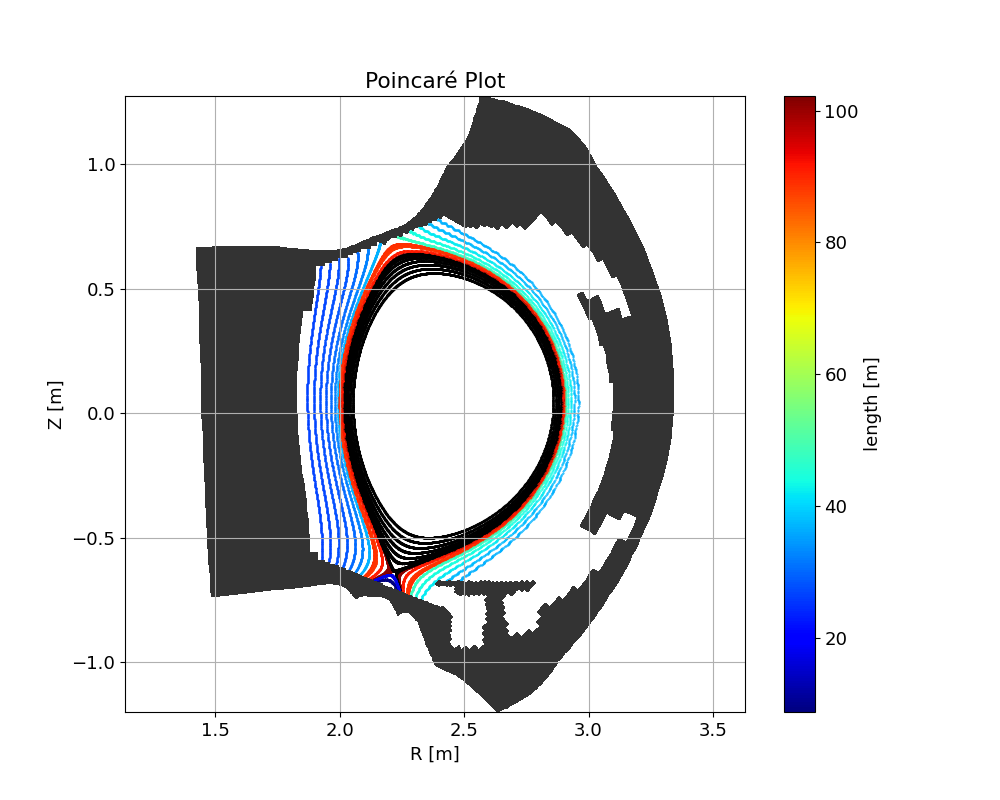
\includegraphics[width=1\textwidth]{schemes/WESTpoincareFull.png}
		\subcaption{Full poloidal plane }
		\label{fig:poincareFull}
	\end{subfigure}
	\begin{subfigure}[t]{0.49\textwidth}
		\centering
		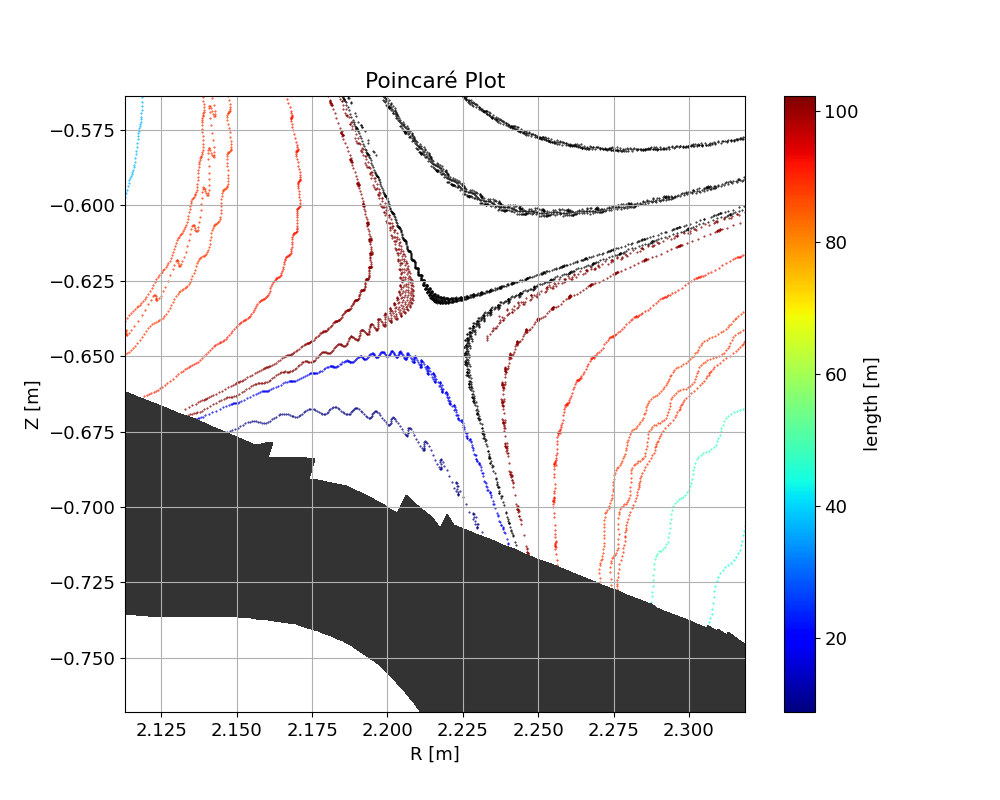
\includegraphics[width=1\textwidth]{schemes/WESTpoincareXpt.png}
		\subcaption{Zoom on the X-point region }		
		\label{fig:poincareXpt}
	\end{subfigure}
	\caption{Poincaré plot at coil-aligned poloidal planes. Seed points are uniformly distributed on the mid-plane along the radial and toroidal directions. Because of the periodicity of the perturbated field, each point corresponds to a field line crossing any of the $N_c$ planes aligned with a coil. The total length of a field line from wall to wall translates in its color, black standing for an infinite closed field line.}
	\label{fig:poincare}
\end{figure}




\section{Application to a WEST scenario}
To demonstrate the newly implemented feature, we perform a SOLEDGE3X simulation on a WEST scenario with ripple. We consider a simple deuterium plasma with recycling fluid neutrals (recycling coefficient 98\%). The core density fixed tp $2\times 10^{19}$ particles/m$^3$, and 1 MW Ohmic heating is equally applied to electrons and ions. Cross-field transport is emulated by a constant diffusion of $0.3$ m$^2$/s. \newline

To reduce numerical costs, we only simulate one ripple period, or 1/18th of the full torus, and periodically expand the simulated plasma in the toroidal direction. The simulation contains 250,000 cells spread over 16 poloidal planes and was run on 384 processors of the MARCONI computing center\cite{iannone2018marconi-fusion} for 20 ms simulated plasma time. The plasma has not yet reached a converged state, but is sufficiently stable to observe ripple-induced phenomena.

\begin{figure}[H]
	\centering
	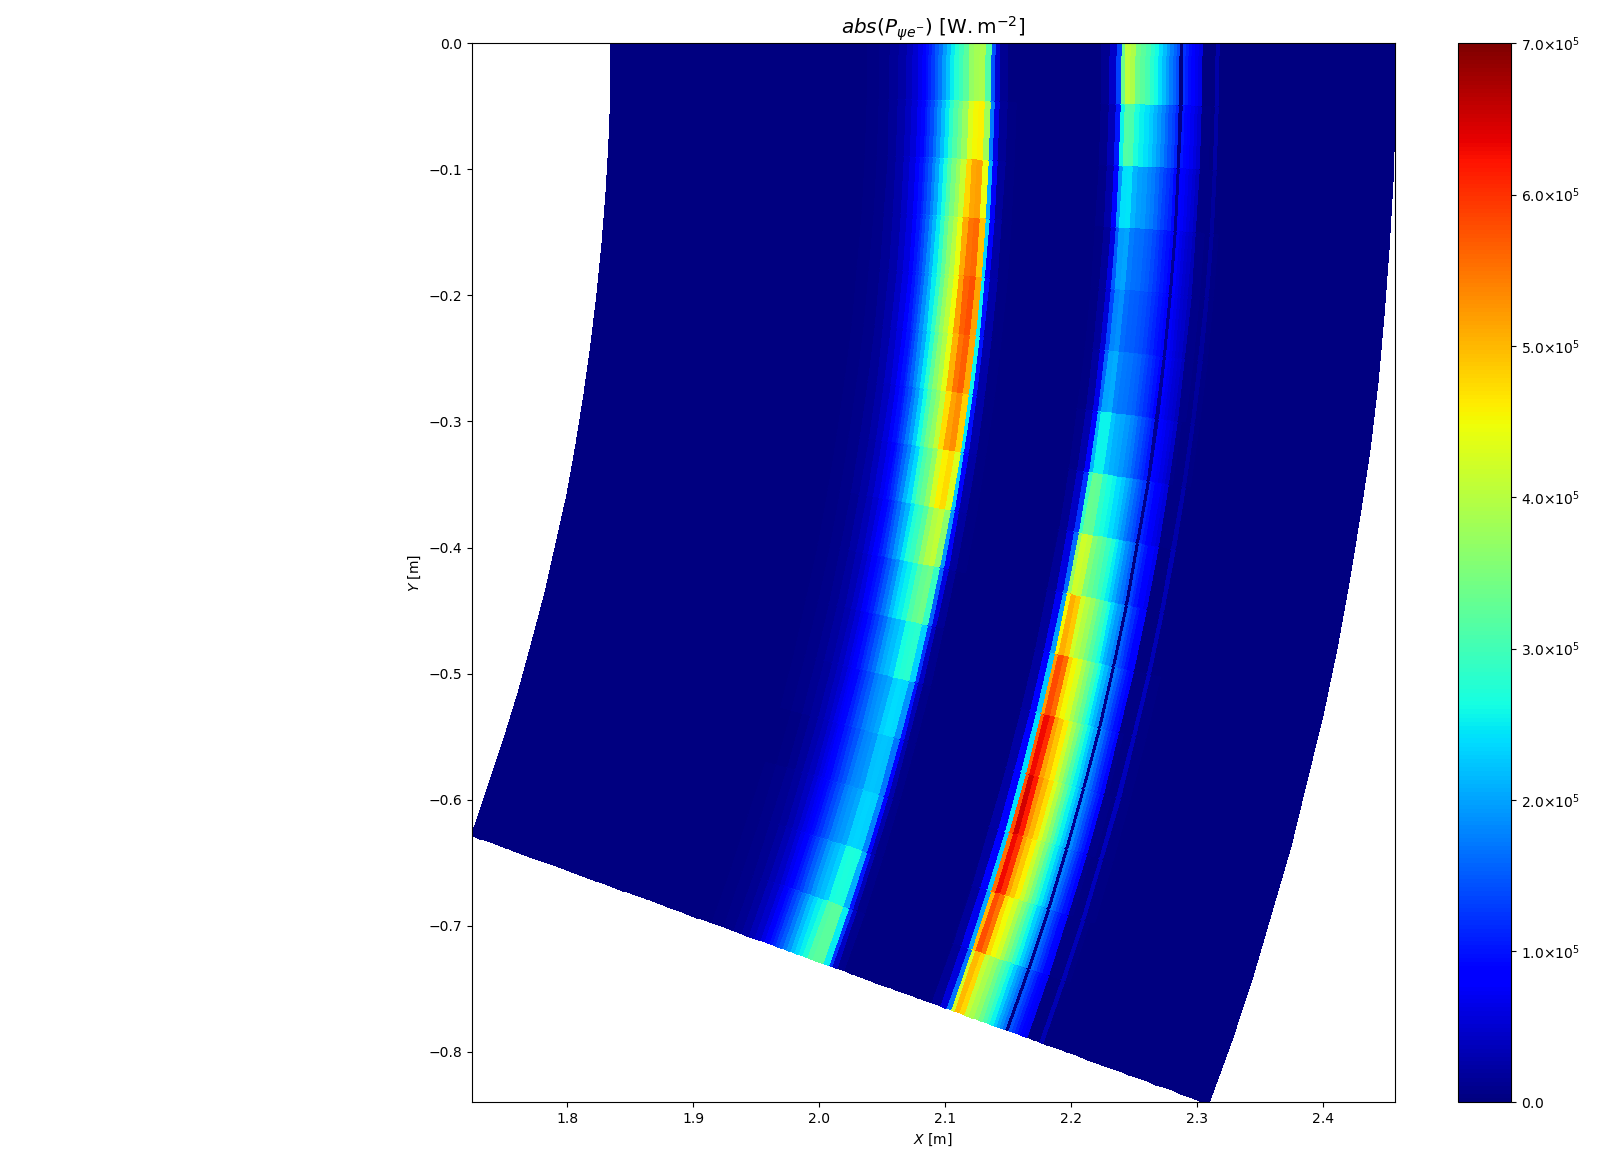
\includegraphics[width=0.48\textwidth]{schemes/WESTripple_targetHeatFlux.png}
	\caption{Calculated electron wall heat flux in the divertor region from the SOLEDGE3X simulation. View on the target from the top for one ripple period.}
	\label{fig:target_S3X}
\end{figure}

In Figure \ref{fig:target_S3X}, the heat fluxes originating at the core source reach the divertor target with maximal heat loads that alternate between the inner and the outer strike point with the toroidal coordinate. It has a strong ressemblance with the "snake skin" pattern in Figure \ref{fig:IR_WEST} observed on infrared imagery during the tokamak operation. 


\section{Conclusion}
The incorporation of magnetic ripple perturbations into the SOLEDGE3X framework significantly enhances its capability to simulate complex magnetic configurations in tokamaks. Using the Biot-Savart law to calculate the ripple effects, this study exhibits the impact of the toroidal magnetic ripple on the magnetic equilibrium configuration in the WEST tokamak. These perturbations both affect the poloidal and the radial component of the axisymmetric magnetic equilibrium, with an important modulation of the poloidal field. \newline

The perturbed magnetic field has been integrated into all parallel advection and gradient terms of the SOLEDGE3X transport model. The radial component of the poloidal perturbation field required major refactoring of the transport model because the mesh remains aligned to axisymmetric flux surfaces. Parallel fluxes now occur in all three directions in the curvilinear coordinates. Consequently, implicit solvers for the heat and viscosity problems are now applied to full-domain 3D systems instead of independent 2D systems on each flux surface, resulting in additional computational costs. \newline

Simulations on a realistic WEST geometry demonstrate the new capability to perform simulations in a non-axisymmetric magnetic configuration. Key features of magnetic ripple, such as the modulation of heat loads on the divertor strike points along the toroidal coordinate, are successfully recovered. \newline

With this new implementation, it will be possible to explore new physics, such as ripple effects on tungsten core contamination or improved predictions of power exhaust in tokamaks. Additionally, this enhancement allows for better comparisons between simulation and experimental data due to the toroidal locality of several plasma diagnostics.
